% ==================================================================
%  §10.1  闭区间上的二重积分
%  源：徐森林、薛春华《数学分析》第二册, 印刷页 183-198
%  底本：PaddleOCR-VL 为主, MinerU 交叉核对
%  约定：全西文标点; \[\] 表行间公式; align*/aligned 表多行;
%        定理/证明以 \qedhere 收 □, 不需 □ 的用 \noqedhere 抑制
%        章节标题（\chapter/\section）按原书原文保留顿号「、」,
%        正文一律不得出现中文标点（规范 §1.3）
%  图：图 10.1.1、10.1.2、10.1.3 原生 TikZ 绘制
% ==================================================================

\section{闭区间上的二重积分}\label{sec:10.1}

回忆一元函数的 Riemann 积分
\[
  \int_{a}^{b} f(x)\,\mathrm{d}x = \lim_{\|T\| \to 0} \sum_{i=1}^{n} f(\xi_{i})\Delta x_{i},
\]
其中 $T\colon a = x_{0} < x_{1} < \cdots < x_{n} = b$ 为 $[a, b]$ 的一个分割, $\|T\| = \max\limits_{1 \leqslant i \leqslant n} \Delta x_{i}$, $\Delta x_{i} = x_{i} - x_{i-1}$, $\xi_{i} \in [x_{i-1}, x_{i}],\, i = 1, 2, \cdots, n$.

为研究二重积分, 设 $\Omega \subset \mathbb{R}^2$ 为有界点集, 非负函数 $f\colon \Omega \to \mathbb{R}$ 的图像 $\operatorname{graph} f = \{(x, y, f(x, y)) \mid (x, y) \in \Omega\}$ 是分布在 $\Omega$ 上的一块曲面 (\cref{fig:10.1.1}). 由 $\Omega$ 和这块曲面 (称为曲顶) 夹成的一个曲顶柱体 (\cref{fig:10.1.1}) 可表示为
\[
  \{(x, y, z) \mid 0 \leqslant z \leqslant f(x, y),\, (x, y) \in \Omega\}.
\]
为计算这个柱体的体积, 将 $\Omega$ 分割成若干小块, 记为 $\Omega_1, \Omega_2, \cdots, \Omega_k$ (\cref{fig:10.1.2}). 任取 $\boldsymbol{\xi}^i \in \Omega_i$, 并用
\[
  \sum_{i=1}^{k} f(\boldsymbol{\xi}^{i}) v(\Omega_{i})
\]
表示曲顶柱体体积的一个近似值, 其中 $v(\Omega_{i})$ 为小块 $\Omega_{i}$ 的面积. 为得到柱体体积的精确值, 应当将分割 $T = \{\Omega_{1}, \Omega_{2}, \cdots, \Omega_{k}\}$ 无限地加细, 并定义曲顶柱体的体积为
\[
  V = \lim_{\|T\| \to 0} \sum_{i=1}^{k} f(\boldsymbol{\xi}^{i}) v(\Omega_{i}),
\]
这里 $\|T\| = \max\{\operatorname{diam}\Omega_1, \operatorname{diam}\Omega_2, \cdots, \operatorname{diam}\Omega_k\}$. 要求上述极限存在有限且不依赖于 $\Omega_i$ 与 $\boldsymbol{\xi}^i$ 的选取. 记
\[
  V = \iint\limits_{\Omega} f(x, y)\,\mathrm{d}x\mathrm{d}y
\]
或
\[
  V = \iint\limits_{\Omega} f(\boldsymbol{x})\,\mathrm{d}v, \quad \boldsymbol{x} = (x, y).
\]
$\mathrm{d}v = \mathrm{d}x\mathrm{d}y$ 称为面积元. 在不致混淆时, 简记为 $V = \int_{\Omega} f$.

\begin{figure}[htbp]
\centering
\begin{minipage}[b]{0.52\linewidth}
\centering
\begin{tikzpicture}[scale=1.1, >=stealth]
  % 坐标轴
  \draw[->, thick] (0,0) -- (0,3.3) node[left] {$z$};
  \draw[->, thick] (0,0) -- (3.2,0) node[below] {$y$};
  \draw[->, thick] (0,0) -- (-1.8,-1.2) node[below left] {$x$};
  \node[above left] at (0,0) {$O$};

  % 虚线轴穿过 Omega 内部
  \draw[dashed] (-0.8,-0.53) -- (0,0);
  \draw[dashed] (0,0) -- (0,1.8);
  \draw[dashed] (0,0) -- (1.8,0);

  % 底面轮廓 Omega
  \def\basepath{
    (-1.4,-0.9) .. controls (-1.8,-0.2) and (-1.2,0.8) .. (-0.1,0.7)
    .. controls (1.0,0.6) and (2.1,0.3) .. (2.1,-0.5)
    .. controls (2.1,-1.2) and (1.2,-0.5) .. (0.7,-0.9)
    .. controls (0.2,-1.3) and (-0.8,-1.4) .. (-1.4,-0.9)
  }
  \draw[thick] \basepath;
  \node at (0.2,-0.8) {$\Omega$};

  % 顶面轮廓曲面
  \def\toppath{
    (-1.4,1.1) .. controls (-1.8,1.9) and (-1.2,2.7) .. (-0.1,2.6)
    .. controls (1.0,2.5) and (2.1,2.3) .. (2.1,1.4)
    .. controls (2.1,0.7) and (1.2,1.3) .. (0.7,0.9)
    .. controls (0.2,0.5) and (-0.8,0.5) .. (-1.4,1.1)
  }
  
  % 侧面母线
  \draw[thick] (-1.55, -0.45) -- (-1.55, 1.55);
  \draw[thick] (2.1, -0.5) -- (2.1, 1.4);
  \draw[thick] (0.7, -0.9) -- (0.7, 0.9);

  % 顶面曲面轮廓
  \draw[thick] \toppath;
  \draw[thick] (-1.4,1.1) .. controls (-0.8,1.5) and (0.6,1.4) .. (2.1,1.4);
  
  % 曲顶文字
  \node[above] at (0.8, 2.7) {曲顶\quad $z=f(x,y)$};
  \draw[->] (0.4, 2.7) .. controls (-0.2, 2.5) .. (-0.1, 2.2);

  % 小柱体 (微元)
  \coordinate (b1) at (1.0, -0.4);
  \coordinate (b2) at (1.3, -0.3);
  \coordinate (b3) at (1.2, -0.55);
  \coordinate (b4) at (0.9, -0.65);
  \draw[thick] (b1) -- (b2) -- (b3) -- (b4) -- cycle;

  \coordinate (t1) at (1.0, 1.7);
  \coordinate (t2) at (1.3, 1.8);
  \coordinate (t3) at (1.2, 1.55);
  \coordinate (t4) at (0.9, 1.45);
  \draw[thick] (t1) -- (t2) -- (t3) -- (t4) -- cycle;

  \draw[dashed] (b1) -- (t1);
  \draw[thick] (b2) -- (t2);
  \draw[thick] (b3) -- (t3);
  \draw[thick] (b4) -- (t4);
\end{tikzpicture}
\caption{}\label{fig:10.1.1}
\end{minipage}
\hfill
\begin{minipage}[b]{0.45\linewidth}
\centering
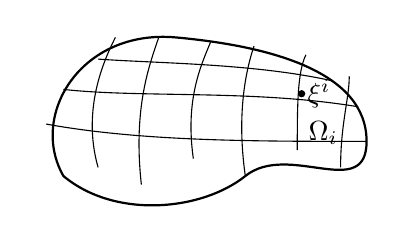
\begin{tikzpicture}[scale=1.1, >=stealth]
  \def\basepathB{
    (-1.4,-0.9) .. controls (-1.8,-0.2) and (-1.2,0.8) .. (-0.1,0.7)
    .. controls (1.0,0.6) and (2.1,0.3) .. (2.1,-0.5)
    .. controls (2.1,-1.2) and (1.2,-0.5) .. (0.7,-0.9)
    .. controls (0.2,-1.3) and (-0.8,-1.4) .. (-1.4,-0.9)
  }
  \draw[thick] \basepathB;

  % 内部网格线
  \draw (-1.0,-0.8) .. controls (-1.2,-0.1) and (-0.9,0.5) .. (-0.8,0.7);
  \draw (-0.5,-1.0) .. controls (-0.6,-0.1) and (-0.4,0.4) .. (-0.3,0.7);
  \draw (0.1,-0.7) .. controls (0.0,0.0) and (0.2,0.4) .. (0.3,0.65);
  \draw (0.7,-0.9) .. controls (0.6,-0.2) and (0.7,0.3) .. (0.8,0.6);
  \draw (1.3,-0.6) .. controls (1.3, -0.1) and (1.3,0.3) .. (1.4,0.5);
  \draw (1.8,-0.8) .. controls (1.8,-0.3) and (1.9,0.0) .. (1.9,0.25);

  \draw (-1.6,-0.3) .. controls (-0.5,-0.5) and (0.8,-0.5) .. (2.1,-0.5);
  \draw (-1.4,0.1) .. controls (-0.5,0.0) and (0.8,0.1) .. (2.0,-0.1);
  \draw (-1.0,0.45) .. controls (-0.3,0.4) and (0.8,0.4) .. (1.7,0.2);

  \node at (1.55, 0.05) {$\boldsymbol{\xi}^i$};
  \fill (1.35, 0.05) circle (1.2pt);
  \node at (1.6, -0.4) {$\Omega_i$};
\end{tikzpicture}
\caption{}\label{fig:10.1.2}
\end{minipage}
\end{figure}

对照一元函数积分的定义, 将 $[a, b]$ 分割成若干子区间, 计算这些区间的长度十分容易. 但是, 在 $\mathbb{R}^{2}$ 中, 一个点集 $\Omega$ 即使有界, 也可能相当复杂. 如何分割 $\Omega$, 如何确定面积 $v(\Omega_i)$, 这是建立二重积分精确定义的最大障碍. 为克服这些障碍, 我们分成两步: 首先讨论二维闭区间上的二重积分, 然后再讨论 $\mathbb{R}^{2}$ 中任一有界集上的二重积分.

\begin{definition}\label{def:10.1.1}
设 $I = [a, b] \times [c, d]$ 为 $\mathbb{R}^{2}$ 中的闭区间 (即每边平行于坐标轴的闭矩形 (闭长方形)). 作 $[a, b]$ 的分割
\[
  T_{x}\colon a = x_{0} < x_{1} < \cdots < x_{n} = b;
\]
又作 $[c, d]$ 的分割
\[
  T_{y}\colon c = y_{0} < y_{1} < \cdots < y_{m} = d.
\]
两族平行直线 $x = x_{i}\,(i = 0, 1, \cdots, n)$ 与 $y = y_{j}\,(j = 0, 1, \cdots, m)$ 将 $I$ 分割成 $k = n \times m$ 个子区间
\[
  [x_{i-1}, x_{i}] \times [y_{j-1}, y_{j}], \quad i = 1, \cdots, n;\; j = 1, \cdots, m.
\]
这 $k$ 个子区间的全体组成 $I$ 的一个分割 $T = T_x \times T_y = \{I_1, I_2, \cdots, I_k\}$. 任取 $\boldsymbol{\xi}^i \in I_i\, (i = 1, 2, \cdots, k)$. 对二元函数 $f\colon I \to \mathbb{R}$ 作 Riemann 和 (也称为积分和)
\[
  \sum_{i=1}^{k} f(\boldsymbol{\xi}^{i}) v(I_{i}),
\]
其中 $v(I_{i})$ 为二维闭区间 (闭矩形) $I_{i}$ 的面积, 即 $I_{i}$ 的长与宽之积. 记
\[
  \|T\| = \max\{\operatorname{diam}I_{1}, \operatorname{diam}I_{2}, \cdots, \operatorname{diam}I_{k}\},
\]
这里 $I_{i}$ 的直径 $\operatorname{diam}I_{i}$ 为矩形 $I_{i}$ 的对角线的长度. 称 $\|T\|$ 为分割 $T$ 的模或宽度. 称 $\boldsymbol{\xi} = (\boldsymbol{\xi}^{1}, \boldsymbol{\xi}^{2}, \cdots, \boldsymbol{\xi}^{k}) \in I_{1} \times I_{2} \times \cdots \times I_{k}$ 为上述 Riemann 和的值点向量, 称 $\boldsymbol{\xi}^{1}, \boldsymbol{\xi}^{2}, \cdots, \boldsymbol{\xi}^{k}$ 为值点.

如果 $\exists J \in \mathbb{R}$, s.t. $\forall \varepsilon > 0$, $\exists \delta > 0$, 当 $\|T\| < \delta$ 时, $\forall \boldsymbol{\xi} \in I_1 \times I_2 \times \cdots \times I_k$, 都有
\[
  \left|\sum_{i=1}^{k} f(\boldsymbol{\xi}^{i}) v(I_{i}) - J\right| < \varepsilon,
\]
则称二元函数 $f$ 在闭区间 $I$ 上 (Riemann) 可积, 而
\[
  J = \lim_{\|T\| \to 0} \sum_{i=1}^{k} f(\boldsymbol{\xi}^{i}) v(I_{i}) \reason{def} \iint_{I} f(x, y)\,\mathrm{d}x\mathrm{d}y \quad\text{或}\quad \int_{I} f\,\mathrm{d}v \quad\text{或}\quad \int_{I} f
\]
称为 $f$ 在 $I$ 上的二重积分, 或简称为 $f$ 在 $I$ 上的积分. 这里 $f$ 称为被积函数, $I$ 称为积分区间, $\mathrm{d}x\mathrm{d}y$ 与 $\mathrm{d}v$ 称为面积元.
\end{definition}

如此定义的积分具有与一元函数积分类似的简单性质.

\begin{theorem}\label{thm:10.1.1}
\begin{enumerate}
  \item $\displaystyle\int_{I} c = c v(I),\, c \in \mathbb{R}$;
  \item 设 $f$ 在二维闭区间 $I \subset \mathbb{R}^2$ 上可积, 则 $\forall c \in \mathbb{R}$ ($c$ 为常数), $cf$ 也可积, 且
  \[
    \int_{I} c f = c\int_{I} f.
  \]
  \item 设 $f_{1}$ 与 $f_{2}$ 在 $I$ 上都可积, 则 $f_{1} + f_{2}$ 在 $I$ 上也可积, 且
  \[
    \int_{I}(f_{1}+f_{2}) = \int_{I} f_{1} + \int_{I} f_{2}.
  \]
  \item 设 $f \geqslant 0$ 且在 $I$ 上可积, 则 $\displaystyle\int_{I} f \geqslant 0$. 特别地, 如果 $f_{1}, f_{2}$ 都在 $I$ 上可积, 且 $f_{1} \geqslant f_{2}$, 则 $\displaystyle\int_{I} f_{1} \geqslant \int_{I} f_{2}$.
  \item 设 $f$ 在 $I$ 上可积, 则 $|f|$ 在 $I$ 上也可积, 且
  \[
    \left|\int_{I} f\right| \leqslant \int_{I} |f|.
  \]
\end{enumerate}
\end{theorem}

\begin{proof}
(1) 因为
\[
  \sum_{i=1}^{k} c v(I_{i}) = c \sum_{i=1}^{k} v(I_{i}) = c v(I),
\]
所以根据积分定义知 $\displaystyle\int_{I} c = c v(I)$.

(2) 因为
\[
  \sum_{i=1}^{k} c f(\boldsymbol{\xi}^{i}) v(I_{i}) = c \sum_{i=1}^{k} f(\boldsymbol{\xi}^{i}) v(I_{i}),
\]
所以根据积分定义知 $\displaystyle\int_{I} c f = c\int_{I} f$.

(3) 因为
\[
  \sum_{i=1}^{k}(f_{1}+f_{2})(\boldsymbol{\xi}^{i}) v(I_{i}) = \sum_{i=1}^{k} f_{1}(\boldsymbol{\xi}^{i}) v(I_{i}) + \sum_{i=1}^{k} f_{2}(\boldsymbol{\xi}^{i}) v(I_{i}),
\]
所以根据积分定义知 $\displaystyle\int_{I}(f_{1}+f_{2}) = \int_{I} f_{1} + \int_{I} f_{2}$.

(4) 因为 $\displaystyle\sum_{i=1}^{k} f(\boldsymbol{\xi}^{i}) v(I_{i}) \geqslant 0$, 故必有 $\displaystyle\int_{I} f \geqslant 0$. (反证) 假设 $\displaystyle\int_{I} f < 0$, 取 $\varepsilon_{0} = -\dfrac{1}{2}\int_{I} f > 0$, 根据 $f$ 可积与积分定义知, $\exists \delta > 0$, 当 $\|T\| < \delta$ 时, 有
\[
  0 \leqslant \sum_{i=1}^{k} f(\boldsymbol{\xi}^{i}) v(I_{i}) < \int_{I} f + \varepsilon_{0} = \int_{I} f - \frac{1}{2}\int_{I} f = \frac{1}{2}\int_{I} f < 0,
\]
矛盾.

特别地, 当 $f_{1} \geqslant f_{2}$ 时, $f_{1} - f_{2} \geqslant 0$. 由上得到
\[
  \int_{I} f_{1} - \int_{I} f_{2} = \int_{I}(f_{1}-f_{2}) \geqslant 0 \implies \int_{I} f_{1} \geqslant \int_{I} f_{2}.
\]

(5) 类似\extref{例 6.1.9} 应用\cref{thm:10.1.7}的 (3) 或 (8) 知, $f$ 可积蕴涵着 $|f|$ 可积. 再由 $-|f| \leqslant f \leqslant |f|$ 及 (4) 立得
\[
  -\int_{I} |f| \leqslant \int_{I} f \leqslant \int_{I} |f|, \quad \text{即} \quad \left|\int_{I} f\right| \leqslant \int_{I} |f|. \qedhere
\]
\end{proof}

\begin{theorem}[惟一性]\label{thm:10.1.2}
设 $f$ 在闭区间 $I = [a, b] \times [c, d]$ 上可积, 则积分值 $J = \displaystyle\int_{I} f$ 是惟一的.
\end{theorem}

\begin{proof}
仿照\extref{定理 6.1.1}证明.
\end{proof}

\begin{theorem}[可积的必要条件]\label{thm:10.1.3}
设 $f$ 在闭区间 $I = [a, b] \times [c, d]$ 上可积, 则 $f$ 在 $I$ 上有界 (因而无界函数不是可积的). 但反之不真.
\end{theorem}

\begin{proof}
仿照\extref{定理 6.1.2}的证明. 只需将反例改为
\[
  f(x, y) = D(x, y) = \begin{cases}
    1, & (x, y) \in \mathbb{Q}^{2} \cap [0, 1]^{2}, \\
    0, & (x, y) \in [0, 1]^{2} \setminus \mathbb{Q}^{2}.
  \end{cases} \qedhere
\]
\end{proof}

与一元函数一样, \cref{thm:10.1.3}只是可积的必要条件, 它只能否定无界函数是可积的, 但对有界函数是否可积就束手无策了. 要判断一个函数是否可积, 原则上可以根据定义直接考察 Riemann 和是否无限接近某个常数 $J$. 但由于常数 $J$ 不易预知及 Riemann 和的复杂性, 这种判断是非常困难的.

为给出 $f$ 在 $I = [a, b] \times [c, d]$ 上可积的充要条件, 先引进零面积集、零测集的概念.

\begin{definition}\label{def:10.1.2}
设 $A \subset \mathbb{R}^{2}$. 如果对任何 $\varepsilon > 0$, 存在有限个闭区间 $I_{1}, I_{2}, \cdots, I_{k}$ 使得 $\bigcup\limits_{i=1}^{k} I_{i} \supseteq A$, 且 $\sum\limits_{i=1}^{k} v(I_{i}) < \varepsilon$, 则称 $A$ 为\textbf{零面积集}.

设 $A \subset \mathbb{R}^{2}$. 如果对任何 $\varepsilon > 0$, 存在至多可数个二维闭区间 $I_{1}, I_{2}, \cdots, I_{k}, \cdots$, 使得 $\bigcup\limits_{i=1}^{\infty} I_{i} \supseteq A$, 且 $\sum\limits_{i=1}^{\infty} v(I_{i}) < \varepsilon$, 则称 $A$ 为\textbf{零测集}.
\end{definition}

该定义中将「闭区间」改为「开区间」, 或「闭圆」, 或「开圆」都是等价的.

\begin{theorem}\label{thm:10.1.4}
零面积集必为零测集, 但反之不真.
\end{theorem}

\begin{proof}
如果 $A \subset \mathbb{R}^{2}$ 为零面积集, 则对任何 $\varepsilon > 0$, 必有二维闭区间 $I_{1}, I_{2}, \cdots, I_{k}$ 使 $\bigcup\limits_{i=1}^{k} I_{i} \supset A$, 且 $\sum\limits_{i=1}^{k} v(I_{i}) < \varepsilon$. 再选面积充分小的 $I_{k+1}, I_{k+2}, \cdots$, 使 $\sum\limits_{i=1}^{\infty} v(I_{i}) < \varepsilon$. 而 $\bigcup\limits_{i=1}^{\infty} I_{i} \supset \bigcup\limits_{i=1}^{k} I_{i} \supset A$ 是显然的. 因此, $A$ 为零测集.

\textbf{反例}: $[0, 1]^{2}$ 中有理点的全体 $\mathbb{Q}^{2} \cap [0, 1]^{2} = \{P^{i} \mid i \in \mathbb{Z}_{+}\}$ 为零测集, 但非零面积集. 作以 $P_i$ 为中心, $\dfrac{\sqrt{\varepsilon}}{2^i}$ 为边长的正方形 $I_i$, 则
\[
  \bigcup_{i=1}^{\infty} I_i \supset \bigcup_{i=1}^{\infty} \{P^i\} = \mathbb{Q}^{2} \cap [0, 1]^{2},
\]
且
\[
  \sum_{i=1}^{\infty} v(I_i) = \sum_{i=1}^{\infty} \left(\frac{\sqrt{\varepsilon}}{2^i}\right)^2 = \sum_{i=1}^{\infty} \frac{\varepsilon}{2^{2i}} = \sum_{i=1}^{\infty} \left(\frac{1}{4}\right)^i \varepsilon = \frac{\varepsilon}{3} < \varepsilon.
\]
由此推得 $\mathbb{Q}^{2} \cap [0, 1]^{2}$ 为零测集. 但它为非零面积集. (反证) 假设 $\mathbb{Q}^{2} \cap [0, 1]^{2}$ 为零面积集, 则对 $\varepsilon_0 = \dfrac{1}{2}$ 存在闭区间 $I_1, I_2, \cdots, I_k$ 使得 $\bigcup\limits_{i=1}^{k} I_i \supset \mathbb{Q}^{2} \cap [0, 1]^{2}$, 且 $\sum\limits_{i=1}^{k} v(I_i) < \varepsilon_0 = \dfrac{1}{2}$. 显然,
\[
  [0, 1]^{2} = \overline{\mathbb{Q}^{2} \cap [0, 1]^{2}} \subset \overline{\bigcup_{i=1}^{k} I_i} = \bigcup_{i=1}^{k} \overline{I_i} = \bigcup_{i=1}^{k} I_i,
\]
所以
\[
  1 = v([0, 1]^{2}) \leqslant v\left(\bigcup_{i=1}^{k} I_i\right) \leqslant \sum_{i=1}^{k} v(I_i) < \varepsilon_0 = \frac{1}{2},
\]
矛盾.
\end{proof}

\begin{example}\label{ex:10.1.1}
设 $f\colon [a, b] \to \mathbb{R}$ 为连续函数, 则集合 ($f$ 的图像)
\[
  \operatorname{graph} f = \{(x, f(x)) \mid x \in [a, b]\} \subset \mathbb{R}^{2}
\]
为零面积集.
\end{example}

\begin{proof}
任给 $\varepsilon > 0$, 因 $f$ 在 $[a, b]$ 上连续, 故一致连续. 于是, 存在 $[a, b]$ 的一个分割: $a = x_{0} < x_{1} < \cdots < x_{n} = b$, 当 $t_{1}, t_{2} \in [x_{i-1}, x_{i}]\, (i = 1, 2, \cdots, n)$ 时,
\[
  |f(t_{1}) - f(t_{2})| < \frac{\varepsilon}{b - a}.
\]
令 $m_{i} = \min f([x_{i-1}, x_{i}])$, $M_{i} = \max f([x_{i-1}, x_{i}])$, 则
\[
  0 \leqslant M_{i} - m_{i} < \frac{\varepsilon}{b - a}, \quad i = 1, 2, \cdots, n.
\]
设 $I_{i} = [x_{i-1}, x_{i}] \times [m_{i}, M_{i}]\, (i = 1, 2, \cdots, n)$. 显见 (\cref{fig:10.1.3}), $\operatorname{graph} f \subset \bigcup\limits_{i=1}^{n} I_{i}$, 且
\[
  \sum_{i=1}^{n} v(I_{i}) < \sum_{i=1}^{n}(x_{i} - x_{i-1}) \cdot \frac{\varepsilon}{b - a} = (b - a) \cdot \frac{\varepsilon}{b - a} = \varepsilon.
\]
因此, $\operatorname{graph} f$ 为零面积集.
\end{proof}

\begin{figure}[htbp]
\centering
\begin{tikzpicture}[scale=1.15, >=stealth]
  % 坐标轴
  \draw[->, thick] (-0.3,0) -- (6.0,0) node[below] {$x$};
  \draw[->, thick] (0,-0.3) -- (0,4.2) node[left] {$y$};

  % 各个竖直立柱的侧边界
  \draw[thick] (0.8,0) -- (0.8,2.0);
  \draw[thick] (1.7,0) -- (1.7,2.0);
  \draw[thick] (2.6,0) -- (2.6,2.2);
  \draw[thick] (3.5,0) -- (3.5,2.7);
  \draw[thick] (4.5,0) -- (4.5,3.6);
  \draw[thick] (5.4,0) -- (5.4,3.6);

  % 绘制每个柱体顶部的矩形 I_i [m_i, M_i] 并填充斜线阴影
  \fill[pattern=north east lines] (0.8,1.8) rectangle (1.7,2.0);
  \draw[thick] (0.8,1.8) rectangle (1.7,2.0);

  \fill[pattern=north east lines] (1.7,1.7) rectangle (2.6,1.9);
  \draw[thick] (1.7,1.7) rectangle (2.6,1.9);

  \fill[pattern=north east lines] (2.6,1.8) rectangle (3.5,2.2);
  \draw[thick] (2.6,1.8) rectangle (3.5,2.2);

  \fill[pattern=north east lines] (3.5,2.1) rectangle (4.5,2.7);
  \draw[thick] (3.5,2.1) rectangle (4.5,2.7);

  \fill[pattern=crosshatch] (4.5,2.6) rectangle (5.4,3.6);
  \draw[thick] (4.5,2.6) rectangle (5.4,3.6);

  % 函数曲线 y = f(x)
  \draw[very thick] (0.8,1.95) .. controls (1.2,1.82) and (1.5,1.75) .. (2.1,1.72)
    .. controls (2.6,1.75) and (3.0,1.95) .. (3.5,2.18)
    .. controls (4.0,2.4) and (4.3,2.6) .. (4.5,2.8)
    .. controls (4.8,3.1) and (5.2,3.4) .. (5.4,3.55);

  % 指向其中一个小矩形 I_i 的箭头
  \draw[->] (2.7, 3.2) node[above left] {$I_i$} -- (3.8, 2.5);
\end{tikzpicture}
\caption{}\label{fig:10.1.3}
\end{figure}

\begin{example}\label{ex:10.1.2}
设 $l \subset \mathbb{R}^{2}$ 为 $C^{1}$ 参数曲线, 则 $l$ 为零面积集.

更进一步, 设 $l \subset \mathbb{R}^{2}$ 为 $C^{0}$ 参数曲线, 并且其中至少有一个分量有连续的导数, 则 $l$ 为零面积集.
\end{example}

\begin{proof}
设 $l$ 有参数表示 $(x, y) = (x(t), y(t)),\, t \in [\alpha, \beta]$, 其中 $x$ 与 $y$ 为 $[\alpha, \beta]$ 上的连续函数, 不妨再设 $y$ 在 $[\alpha, \beta]$ 上有连续的导数. 由最值定理, $\exists M > 0$, s.t. $|y'(t)| \leqslant M$, $\forall t \in [\alpha, \beta]$. 于是, $\forall \varepsilon > 0$, 由于 $x(t)$ 在 $[\alpha, \beta]$ 上一致连续, 故必有分割
\[
  T\colon \alpha = t_{0} < t_{1} < \cdots < t_{m} = \beta,
\]
s.t. 当 $s, t \in [t_{i-1}, t_i]\, (i = 1, 2, \cdots, m)$ 时, 有
\[
  |x(s) - x(t)| < \frac{\varepsilon}{2M(\beta - \alpha)}.
\]
令
\[
  a_{i} = \min x([t_{i-1}, t_{i}]), \quad b_{i} = \max x([t_{i-1}, t_{i}]),
\]
则有 $b_{i} - a_{i} \leqslant \dfrac{\varepsilon}{2M(\beta - \alpha)}$. 再令
\[
  c_{i} = \min y([t_{i-1}, t_{i}]), \quad d_{i} = \max y([t_{i-1}, t_{i}]),
\]
\[
  I_{i} = [a_{i}, b_{i}] \times [c_{i}, d_{i}], \quad i = 1, 2, \cdots, m.
\]
于是, 当 $t \in [t_{i-1}, t_i]$ 时, $(x(t), y(t)) \in I_i\, (i = 1, 2, \cdots, m)$. 所以
\[
  l \subset \bigcup_{i=1}^{m} I_{i}.
\]
由于 $y(t)$ 在 $[\alpha, \beta]$ 上连续, 根据最值定理, $\exists t_{i}^{(0)}, t_{i}^{(1)} \in [t_{i-1}, t_{i}]$, s.t. $y(t_{i}^{(0)}) = d_{i}$, $y(t_{i}^{(1)}) = c_{i}$. 再由 Lagrange 中值定理, $\exists \theta_{i} \in [t_{i}^{(0)}, t_{i}^{(1)}] \subset [t_{i-1}, t_{i}]$, 有
\begin{align*}
  0 &\leqslant d_{i} - c_{i} = y(t_{i}^{(0)}) - y(t_{i}^{(1)}) = y'(\theta_{i})(t_{i}^{(0)} - t_{i}^{(1)}) \\
    &\leqslant M |t_{i}^{(0)} - t_{i}^{(1)}| \leqslant M(t_{i} - t_{i-1}).
\end{align*}
由此推得
\begin{align*}
  \sum_{i=1}^{m} v(I_{i}) &= \sum_{i=1}^{m}(b_{i} - a_{i})(d_{i} - c_{i}) \leqslant \sum_{i=1}^{m} \frac{\varepsilon}{2M(\beta - \alpha)} M(t_{i} - t_{i-1}) \\
  &= \frac{\varepsilon}{2M(\beta - \alpha)} M(\beta - \alpha) = \frac{\varepsilon}{2} < \varepsilon.
\end{align*}
这就证明了 $l$ 为零面积集.
\end{proof}

\begin{remark}\label{rem:10.1.1}
\begin{enumerate}
  \item 设函数 $f\colon [a, b] \to \mathbb{R}$ 连续, 由\cref{ex:10.1.2}的结论知, $f$ 的图像
  \[
    \operatorname{graph} f = \{(x, f(x)) \mid x \in [a, b]\} = \{(t, f(t)) \mid t \in [a, b]\} \subset \mathbb{R}^{2}
  \]
  为零面积集.
  \item 如果 $x(t), y(t)$ 只连续, 但都不具有连续可导的条件, 则\cref{ex:10.1.2}的结论可能不成立. 甚至我们将在第三册中给出一条连续的参数曲线, 它竟能充满整个正方形, 从而这条连续曲线就不是零面积集.
\end{enumerate}
\end{remark}

关于零面积集与零测集, 还有下面定理.

\begin{theorem}\label{thm:10.1.5}
\begin{enumerate}
  \item 至多可数集为零测集.
  \item 零测集的任何子集为零测集.
  \item 至多可数个零测集 $A_i$ 的并集 $\bigcup\limits_{i} A_i$ 仍为零测集.
  \item 零面积集的任何子集为零面积集.
  \item 有限个零面积集之并仍为零面积集; 可数个零面积集之并未必为零面积集.
  \item $A$ 为零面积集 $\iff \overline{A}$ 也为零面积集.
  \item 如果 $A$ 为有界闭集, 则 $A$ 为零测集 $\iff A$ 为零面积集.
\end{enumerate}
\end{theorem}

\begin{proof}
(1) $\sim$ (4) 和 (5) 的第一结论是显而易见的, 读者自己可以证明. 这里只证 (5) 的第二个论断及 (6), (7).

(5) $\boldsymbol{x} = (x, y) \in \mathbb{R}^{2}$, $\forall \varepsilon > 0$, 作闭区间
\[
  I = \left[x - \frac{\sqrt{\varepsilon}}{4}, x + \frac{\sqrt{\varepsilon}}{4}\right] \times \left[y - \frac{\sqrt{\varepsilon}}{4}, y + \frac{\sqrt{\varepsilon}}{4}\right],
\]
则 $\boldsymbol{x} \in I$, 且 $v(I) = \left(\dfrac{\sqrt{\varepsilon}}{2}\right)^{2} = \dfrac{\varepsilon}{4} < \varepsilon$. 因此, 独点集 $\{\boldsymbol{x}\}$ 为零面积集.

显然, $\mathbb{Q}^2 \cap [0, 1]^2 = \{P^i \mid i \in \mathbb{Z}_+\}$ 为可数个独点集之并, 因而它为可数个零面积集的并. 但根据\cref{thm:10.1.4}证明知, $\mathbb{Q}^2 \cap [0, 1]^2$ 为非零面积集.

(6) ($\Leftarrow$) 因为 $A \subset \overline{A}$, 根据 (4) 知, $\overline{A}$ 为零面积集蕴涵着 $A$ 为零面积集.

($\Rightarrow$) 设 $A$ 为零面积集, 则 $\forall \varepsilon > 0$, 必有闭区间 $I_{1}, I_{2}, \cdots, I_{m}$, s.t.
\[
  A \subset \bigcup_{i=1}^{m} I_{i}, \quad \sum_{i=1}^{m} v(I_{i}) < \varepsilon.
\]
由于 $\bigcup\limits_{i=1}^{m} I_{i}$ 为闭集, 所以仍有
\[
  \overline{A} \subset \overline{\bigcup_{i=1}^{m} I_{i}} = \bigcup_{i=1}^{m} \overline{I_{i}} = \bigcup_{i=1}^{m} I_{i}.
\]
由此可见 $\overline{A}$ 为零面积集.

(7) ($\Leftarrow$) 见\cref{thm:10.1.4}.

($\Rightarrow$) 设 $A$ 为紧致的零测集, 则对任何 $\varepsilon > 0$, 存在开区间序列 $\{I_{i}\}$, 使得
\[
  A \subset \bigcup_{i=1}^{\infty} I_{i} \quad\text{且}\quad \sum_{i=1}^{\infty} v(I_{i}) < \varepsilon.
\]
由有限覆盖定理, 从 $\{I_{i}\}$ 中可选出有限个开区间仍能覆盖住 $A$, 这些开区间面积之和自然仍小于 $\varepsilon$, 所以 $A$ 为零面积集.
\end{proof}

下面将给出 Riemann 可积的充要条件, 它只与被积函数 $f$ 本身有关, 而不涉及 Riemann 积分的值.

设 $f\colon I \to \mathbb{R}$ 为有界函数, $I = [a, b] \times [c, d] \subset \mathbb{R}^2$ 为闭区间, $M = \sup\limits_{\boldsymbol{x} \in I} f(\boldsymbol{x})$, $m = \inf\limits_{\boldsymbol{x} \in I} f(\boldsymbol{x})$. $T = \{I_1, I_2, \cdots, I_k\}$ 为\cref{def:10.1.1}中所述的 $I$ 的一个分割.
\[
  M_{i}^{f} = \sup_{\boldsymbol{x} \in I_{i}} f(\boldsymbol{x}), \quad m_{i}^{f} = \inf_{\boldsymbol{x} \in I_{i}} f(\boldsymbol{x}).
\]
在不致混淆时, 记 $M_{i}^{f}$ 为 $M_{i}$, $m_{i}^{f}$ 为 $m_{i}$.

分别称
\[
  S(T, f) = \sum_{i=1}^{k} M_{i} v(I_{i}) \quad\text{与}\quad s(T, f) = \sum_{i=1}^{k} m_{i} v(I_{i})
\]
为 $f$ 关于分割 $T$ 的 Darboux 上和与 Darboux 下和, 统称为 Darboux 和. 在不致混淆时, 分别记 $S(T, f)$ 与 $s(T, f)$ 为 $S(T)$ 与 $s(T)$. 显然, $\forall \boldsymbol{\xi}^{i} \in I_{i}\,(i = 1, 2, \cdots, k)$, Riemann 和 $S(T, f, \boldsymbol{\xi}) = \sum\limits_{i=1}^{k} f(\boldsymbol{\xi}^{i}) v(I_{i})$ 满足
\[
  m v(I) \leqslant \sum_{i=1}^{k} m_{i} v(I_{i}) \leqslant \sum_{i=1}^{k} f(\boldsymbol{\xi}^{i}) v(I_{i}) \leqslant \sum_{i=1}^{k} M_{i} v(I_{i}) \leqslant M v(I),
\]
即
\[
  m v(I) \leqslant s(T, f) \leqslant S(T, f, \boldsymbol{\xi}) \leqslant S(T, f) \leqslant M v(I),
\]
其中 $\boldsymbol{\xi} = (\boldsymbol{\xi}^{1}, \boldsymbol{\xi}^{2}, \cdots, \boldsymbol{\xi}^{k})$.

设 $\omega_{i}^{f} = M_{i}^{f} - m_{i}^{f}$, 称它为 $f$ 在 $I_{i}$ 上的振幅, 简记为 $\omega_{i} = M_{i} - m_{i}$, 而
\[
  S(T, f) - s(T, f) = \sum_{i=1}^{k}(M_{i} - m_{i}) v(I_{i}) = \sum_{i=1}^{k} \omega_{i} v(I_{i}) \quad \left(\text{或}\quad \sum_{T} \omega_{i} v(I_{i})\right)
\]
称为 $f$ 在 $I$ 上关于分割 $T$ 的振幅和.

\begin{lemma}\label{lem:10.1.1}
对闭区间 $I \subset \mathbb{R}^2$ 的同一分割 $T = \{I_1, I_2, \cdots, I_k\}$, 相对于任何 $\boldsymbol{\xi} = (\boldsymbol{\xi}^1, \boldsymbol{\xi}^2, \cdots, \boldsymbol{\xi}^k) \in I_1 \times I_2 \times \cdots \times I_k$, 有
\[
  S(T, f) = \sup_{\boldsymbol{\xi}} \sum_{i=1}^{k} f(\boldsymbol{\xi}^{i}) v(I_{i}), \quad s(T, f) = \inf_{\boldsymbol{\xi}} \sum_{i=1}^{k} f(\boldsymbol{\xi}^{i}) v(I_{i}).
\]
\end{lemma}

\begin{proof}
仿\extref{引理 6.1.1}证明.
\end{proof}

设 $T' = T_{x}' \times T_{y}'$, $T'' = T_{x}'' \times T_{y}''$ 为闭区间 $I \subset \mathbb{R}^2$ 的两个分割. $T_{x}' + T_{x}''$ 表示将 $T'_{x}$ 与 $T''_{x}$ 的所有分点合并得到的分割 (重复的分点只取一次), $T'_{y} + T''_{y}$ 表示将 $T'_{y}$ 与 $T''_{y}$ 的所有分点合并得到的分割 (重复的分点只取一次). 记 $T' + T'' = (T_{x}' + T''_{x}) \times (T'_{y} + T''_{y})$.

\begin{lemma}\label{lem:10.1.2}
$S(T' + T'') \leqslant S(T')$, $s(T' + T'') \geqslant s(T')$;
\[
  S(T' + T'') \leqslant S(T''), \quad s(T' + T'') \geqslant s(T'').
\]
\end{lemma}

\begin{proof}
类似\extref{引理 6.1.2}的证明知, 分割增加新分点后, 上和不增, 下和不减. 因此, 立即推得引理中的结论.
\end{proof}

\begin{lemma}\label{lem:10.1.3}
对闭区间 $I \subset \mathbb{R}^{2}$ 的任意两个分割 $T'$ 与 $T''$, 有
\[
  s(T') \leqslant S(T'').
\]
\end{lemma}

\begin{proof}
由\cref{lem:10.1.2}便有
\[
  s(T') \leqslant s(T' + T'') \leqslant S(T' + T'') \leqslant S(T''). \qedhere
\]
\end{proof}

\begin{lemma}\label{lem:10.1.4}
$m v(I) \leqslant \sup\limits_{T'} s(T') \leqslant \inf\limits_{T''} S(T'') \leqslant M v(I)$.
\end{lemma}

\begin{proof}
由\cref{lem:10.1.3}知
\[
  m v(I) \leqslant s(T') \leqslant S(T'') \leqslant M v(I),
\]
从而有
\[
  m v(I) \leqslant \sup_{T'} s(T') \leqslant \inf_{T''} S(T'') \leqslant M v(I),
\]
即
\[
  m v(I) \leqslant s \leqslant S \leqslant M v(I),
\]
其中 $S = \inf\limits_{T} S(T)$ 与 $s = \sup\limits_{T} s(T)$ 分别称为 $f$ 在 $I$ 上的上积分与下积分.
\end{proof}

\begin{theorem}[Darboux 定理]\label{thm:10.1.6}
$\lim\limits_{\|T\| \to 0} S(T) = S, \quad \lim\limits_{\|T\| \to 0} s(T) = s$.
\end{theorem}

\begin{proof}
$\forall \varepsilon > 0$, 由 $S$ 的定义知, 必有某个分割 $T' = T_{x}' \times T_{y}'$, s.t.
\[
  S(T') < S + \frac{\varepsilon}{2}.
\]
设 $T_{x}'$ 与 $T_{y}'$ 分别由 $p$ 个与 $q$ 个分点构成. 对于任意另外一个分割 $T$, $(T+T')_{x}$ 至多比 $T_{x}$ 多 $p$ 个分点, $(T+T')_{y}$ 至多比 $T_{y}$ 多 $q$ 个分点. 根据\extref{引理 6.1.2}证明中的方法与\cref{lem:10.1.2}有
\begin{align*}
  S(T) - (M - m)[p(d - c) + q(b - a)] \|T\|
  &\leqslant S(T) - (M - m)[p(d - c)\|T_{x}\| + q(b - a)\|T_{y}\|] \\
  &\leqslant S(T + T') \leqslant S(T').
\end{align*}
于是, 当 $\|T\| < \dfrac{\varepsilon}{2(M - m + 1)[p(d - c) + q(b - a)]}$ 时,
\begin{align*}
  S &\leqslant S(T) \leqslant S(T') + (M - m)[p(d - c) + q(b - a)] \|T\| \\
    &< S(T') + (M - m)[p(d - c) + q(b - a)] \frac{\varepsilon}{2(M - m + 1)[p(d - c) + q(b - a)]} \\
    &< S(T') + \frac{\varepsilon}{2} < \left(S + \frac{\varepsilon}{2}\right) + \frac{\varepsilon}{2} = S + \varepsilon.
\end{align*}
这就证明了 $\lim\limits_{\|T\| \to 0} S(T) = S$.

同理, 或用 $-f$ 代替 $f$ 得到 $\lim\limits_{\|T\| \to 0} s(T) = s$.
\end{proof}

\begin{theorem}[Riemann 可积的充要条件]\label{thm:10.1.7}
设 $I \subset \mathbb{R}^2$ 为闭区间, $f\colon I \to \mathbb{R}$ 为有界函数, 即 $|f(\boldsymbol{x})| \leqslant M$, $\forall \boldsymbol{x} \in I$. 则下面结论等价:
\begin{enumerate}
  \item $f$ 在 $I$ 上 Riemann 可积.
  \item $f$ 在 $I$ 上的上积分与下积分相等, 即 $S = s$.
  \item 对任何 $\varepsilon > 0$, 存在 $I$ 的某个分割 $T$, 使得
  \[
    S(T) - s(T) = \sum_{i=1}^{k} \omega_{i} v(I_{i}) < \varepsilon.
  \]
  \item 存在 $I$ 的分割串 $T_{m}\,(m = 1, 2, \cdots)$, 使得
  \[
    \lim_{m \to +\infty}[S(T_{m}) - s(T_{m})] = 0.
  \]
  \item $\lim\limits_{\|T\| \to 0}[S(T) - s(T)] = 0$.
  \item 对任何 $\varepsilon > 0$, 存在 $I$ 的某个分割 $T$, 使对任何 $\boldsymbol{\xi} = (\boldsymbol{\xi}^{1}, \boldsymbol{\xi}^{2}, \cdots, \boldsymbol{\xi}^{k}) \in I_{1} \times I_{2} \times \cdots \times I_{k}$, 有
  \[
    |S(T, f, \boldsymbol{\xi}) - J| < \varepsilon.
  \]
  \item 对任何 $\varepsilon > 0, \eta > 0$, 存在 $I$ 的某个分割 $T = \{I_{1}, I_{2}, \cdots, I_{k}\}$, 使得
  \[
    \sum_{\omega_{i} \geqslant \varepsilon} v(I_{i}) < \eta.
  \]
  \item \textbf{(Lebesgue 定理)} $f$ 在 $I$ 上几乎处处连续, 即 $f$ 的不连续点集 $D_{\text{不}}^{f}$ (简记为 $D_{\text{不}}$) 为零测集, 记作
  \[
    \operatorname{meas} D_{\text{不}} = 0.
  \]
\end{enumerate}
\end{theorem}

\begin{proof}
我们只证 (3) $\Leftrightarrow$ (8), 其余证明完全仿照\extref{定理 6.1.4}中相应部分的证明.

(3) $\Rightarrow$ (8): 对任何 $\varepsilon > 0$, 存在 $I$ 的某分割 $T = \{I_{1}, I_{2}, \cdots, I_{k}\}$, 使得
\[
  S(T) - s(T) < \frac{\delta}{2} \varepsilon,
\]
其中 $\delta > 0$ 为任何正数. 令
\[
  D_{\delta} = \left\{\boldsymbol{x} \in I \;\middle|\; \omega_{f}(\boldsymbol{x}) = \lim_{r \to 0^{+}} \omega_{f}(\boldsymbol{x}, r) = \lim_{r \to 0^{+}} [\sup f(I \cap B(\boldsymbol{x}; r)) - \inf f(I \cap B(\boldsymbol{x}; r))] \geqslant \delta\right\},
\]
则
\[
  \sum_{D_{\delta} \cap I_{i}^{\circ} \neq \varnothing} v(I_{i}) < \frac{\varepsilon}{2}.
\]
若不然,
\[
  \frac{\delta}{2}\varepsilon > S(T) - s(T) \geqslant \sum_{D_{\delta} \cap I_{i}^{\circ} \neq \varnothing} \omega_{i} v(I_{i}) \geqslant \sum_{D_{\delta} \cap I_{i}^{\circ} \neq \varnothing} \delta v(I_{i}) \geqslant \delta \cdot \frac{\varepsilon}{2} = \frac{\delta}{2}\varepsilon,
\]
矛盾.

显然, $\bigcup\limits_{i=1}^{k} \partial I_{i}$ 为零面积集, 故必有闭区间 $J_{1}, J_{2}, \cdots, J_{m}$, 使得
\[
  \bigcup_{i=1}^{k} \partial I_{i} \subset \bigcup_{j=1}^{m} J_{j}, \quad\text{且}\quad \sum_{j=1}^{m} v(J_{j}) < \frac{\varepsilon}{2}.
\]
由此可知
\[
  D_{\delta} \subset \left(\bigcup_{\omega_{i} \geqslant \delta} I_{i}\right) \bigcup \left(\bigcup_{j=1}^{m} J_{j}\right),
\]
并且
\[
  \sum_{\omega_{i} \geqslant \delta} v(I_{i}) + \sum_{j=1}^{m} v(J_{j}) < \frac{\varepsilon}{2} + \frac{\varepsilon}{2} = \varepsilon.
\]
这就证明了 $D_{\delta}$ 为零测集, 从而由下面的\cref{thm:10.1.8}与\cref{thm:10.1.5}(3) 知, $D_{\text{不}} = \bigcup\limits_{n=1}^{\infty} D_{\frac{1}{n}}$ 为零测集.

(8) $\Rightarrow$ (3): 设 $D_{\text{不}}$ 为零测集. $\forall \varepsilon > 0$, 存在开区间序列 $\{U_{i}\}$, 使得
\[
  D_{\text{不}} \subset \bigcup_{i=1}^{\infty} U_{i}, \quad \sum_{i=1}^{\infty} v(U_{i}) < \frac{\varepsilon}{4M + 1}.
\]
对任何 $\boldsymbol{x} \in I \setminus \bigcup\limits_{i=1}^{\infty} U_{i} \subset I \setminus D_{\text{不}}$, $f$ 在 $\boldsymbol{x}$ 处连续, 故存在 $\boldsymbol{x}$ 的开邻域 $U_{\boldsymbol{x}}$, 使得 $\omega_{f}(U_{\boldsymbol{x}} \cap I) < \dfrac{\varepsilon}{2 v(I)}$.

显然 $\mathcal{J} = \left\{U_{i}, U_{\boldsymbol{x}} \;\middle|\; i = 1, 2, \cdots;\; \boldsymbol{x} \in I \setminus \bigcup\limits_{i=1}^{\infty} U_{i}\right\}$ 为紧致集 $I$ 的一个开覆盖. 根据 Heine-Borel 有限覆盖定理, 存在 $\mathcal{J}$ 的有限子集 $\mathcal{J}' = \{U_{i_{l}}, U_{\boldsymbol{x}^{s}} \mid l = 1, 2, \cdots, p;\; s = 1, 2, \cdots, q\}$ 覆盖 $I$. 再根据 Lebesgue 数定理, 存在 Lebesgue 数 $\lambda = \lambda(\mathcal{J}') > 0$. 当 $I$ 的分割 $T = \{I_{1}, I_{2}, \cdots, I_{k}\}$ 满足 $\|T\| < \lambda$ 时, 必有
\[
  I_{i} \subset U_{i_{l}} \quad\text{或}\quad U_{\boldsymbol{x}^{s}}.
\]
于是
\begin{align*}
  0 &\leqslant S(T) - s(T) = \sum_{i=1}^{k} \omega_{i} v(I_{i}) \\
    &\leqslant \sum_{I_{i} \subset U_{i_{l}}} \omega_{i} v(I_{i}) + \sum_{I_{i} \subset U_{\boldsymbol{x}^{s}}} \omega_{i} v(I_{i}) \\
    &\leqslant 2M \sum_{1} v(I_{i}) + \frac{\varepsilon}{2 v(I)} \sum_{2} v(I_{i}) \\
    &\leqslant 2M \sum_{i=1}^{\infty} v(U_{i}) + \frac{\varepsilon}{2 v(I)} v(I) \\
    &< 2M \cdot \frac{\varepsilon}{4M + 1} + \frac{\varepsilon}{2} < \varepsilon. \qedhere
\end{align*}
\end{proof}

\begin{remark}\label{rem:10.1.2}
我们可以不应用 Darboux 定理证明\cref{thm:10.1.7}中的 (2) $\Rightarrow$ (3).

事实上, 设 $J = S = s$. 由下积分的定义, 对任何 $\varepsilon > 0$, 存在闭区间 $I$ 的一个分割 $T'$, 使得
\[
  s(T') > J - \frac{\varepsilon}{2};
\]
又由上积分的定义, 存在闭区间 $I$ 的一个分割 $T''$, 使得
\[
  S(T'') < J + \frac{\varepsilon}{2}.
\]
于是, 有
\[
  J - \frac{\varepsilon}{2} < s(T') \leqslant s(T' + T'') \leqslant S(T' + T'') \leqslant S(T'') < J + \frac{\varepsilon}{2}.
\]
由此推得
\[
  S(T' + T'') - s(T' + T'') < \left(J + \frac{\varepsilon}{2}\right) - \left(J - \frac{\varepsilon}{2}\right) = \varepsilon.
\]
令 $T = T' + T''$, 它为 $I$ 的一个分割, 且有
\[
  S(T) - s(T) < \varepsilon.
\]
\end{remark}

\begin{theorem}\label{thm:10.1.8}
设 $A \subset \mathbb{R}^{2}$, 则
\[
  \text{函数 } f\colon A \to \mathbb{R} \text{ 在点 } \boldsymbol{x} \in A \text{ 处连续} \iff \omega_f(\boldsymbol{x}) = \lim_{r \to 0^+} \omega_f(\boldsymbol{x}, r) = 0,
\]
其中 $\omega_{f}(\boldsymbol{x}, r) = \sup f(A \cap B(\boldsymbol{x}; r)) - \inf f(A \cap B(\boldsymbol{x}; r))$ 为 $f$ 在 $A \cap B(\boldsymbol{x}; r)$ 上的振幅, 而 $\omega_{f}(\boldsymbol{x})$ 为 $f$ 在点 $\boldsymbol{x}$ 处的振幅.
\end{theorem}

\begin{proof}
与\extref{定理 2.4.6}的证明完全类似.
\end{proof}

\begin{example}\label{ex:10.1.3}
证明 Dirichlet 函数
\[
  D(x, y) = \begin{cases}
    1, & (x, y) \in \mathbb{Q}^{2} \cap [0, 1]^{2}, \\
    0, & (x, y) \in [0, 1]^{2} \setminus \mathbb{Q}^{2}
  \end{cases}
\]
在 $[0, 1]^{2}$ 上不可积.
\end{example}

\begin{proof}
\textbf{证法 1}\quad 类似\extref{定理 6.1.2}中反例的证明.

\textbf{证法 2, 3, 4}\quad 类似\extref{例 6.1.1}中的证法 2, 3, 4.
\end{proof}

\begin{example}\label{ex:10.1.4}
设 $I \subset \mathbb{R}^2$ 为闭区间, $f\colon I \to \mathbb{R}$ 有界. 若 $l = \{\boldsymbol{x} \in I \mid f(\boldsymbol{x}) \neq 0\}$ 为零面积集, 则 $f$ 在 $I$ 上可积, 且 $\displaystyle\int_I f = 0$.
\end{example}

\begin{proof}
\textbf{证法 1}\quad 显然, $I^{\circ} \setminus \overline{l} = I^{\circ} \cap (\mathbb{R}^{2} \setminus \overline{l})$ 中的点为 $f$ 的连续点, 可见 $D_{\text{不}} \subset \partial I \cup \overline{l}$. 由于 $\partial I$ 与 $\overline{l}$ 都为零面积集, 故 $\partial I \cup \overline{l}$ 也为零面积集. 根据 Lebesgue 定理 (\cref{thm:10.1.7}(8)) 知, $f$ 在 $I$ 上可积.

对于 $I$ 的任一分割 $T = \{I_{1}, I_{2}, \cdots, I_{k}\}$. 由于 $\overline{l}$ 为零面积集, 故必 $\exists \boldsymbol{\xi}^{i} \in I_{i}$, s.t. $f(\boldsymbol{\xi}^{i}) = 0\,(i = 1, 2, \cdots, k)$. 此时, Riemann 和
\[
  \sum_{i=1}^{k} f(\boldsymbol{\xi}^{i}) v(I_{i}) = 0.
\]
由积分的存在性立知 $\displaystyle\int_{I} f = 0$.

\textbf{证法 2}\quad 设 $|f(\boldsymbol{x})| < M$, $\forall \boldsymbol{x} \in I$. $\forall \varepsilon > 0$, 因为 $l$ 为零面积集, 故存在闭区间 $J_{1}, J_{2}, \cdots, J_{m}$, 使 $\bigcup\limits_{i=1}^{m} J_{i} \supset l$, 且 $\sum\limits_{i=1}^{m} v(J_{i}) < \dfrac{\varepsilon}{M}$. 将每个 $J_{i}$ 稍稍扩大得到闭区间 $\widetilde{J}_{i}$, 使 $\sum\limits_{i=1}^{m} v(\widetilde{J}_{i}) < \dfrac{\varepsilon}{M}$, 且
\[
  \delta = \rho_{0}^{2}\left(l, \partial\left(\bigcup_{i=1}^{m}\widetilde{J}_{i}\right)\right) = \inf\left\{\rho_{0}^{2}(\boldsymbol{x}, \boldsymbol{y}) = \|\boldsymbol{x} - \boldsymbol{y}\| \;\middle|\; \boldsymbol{x} \in l, \boldsymbol{y} \in \partial\left(\bigcup_{i=1}^{m}\widetilde{J}_{i}\right)\right\} > 0.
\]
设 $T = \{I_{1}, I_{2}, \cdots, I_{k}\}$ 为 $I$ 的一个分割, 且 $\|T\| < \delta$, 则当 $I_{j} \cap l \neq \varnothing$ 时, 必有 $I_{j} \subset \bigcup\limits_{i=1}^{m} \widetilde{J}_{i}$, 所以
\begin{align*}
  |S(T, f, \boldsymbol{\xi}) - 0| &= \left|\sum_{I_{j} \cap l \neq \varnothing} f(\boldsymbol{\xi}^{j}) v(I_{j}) + \sum_{I_{j} \cap l = \varnothing} f(\boldsymbol{\xi}^{j}) v(I_{j})\right| \\
  &= \left|\sum_{I_{j} \cap l \neq \varnothing} f(\boldsymbol{\xi}^{j}) v(I_{j})\right| \leqslant M \sum_{I_{j} \cap l \neq \varnothing} v(I_{j}) \leqslant M \sum_{i=1}^{m} v(\widetilde{J}_{i}) \\
  &< M \cdot \frac{\varepsilon}{M} = \varepsilon,
\end{align*}
从而 $\displaystyle\int_{I} f = \lim_{\|T\| \to 0} S(T, f, \boldsymbol{\xi}) = 0$.
\end{proof}

\begin{remark}\label{rem:10.1.3}
\begin{enumerate}
  \item 从\cref{ex:10.1.4}可知, $\mathbb{Q}^{2} \cap [0, 1]^{2}$ 不为零面积集.
  
  (反证) 假设 $\mathbb{Q}^{2} \cap [0, 1]^{2}$ 为零面积集, 则由\cref{ex:10.1.4}推得 $\mathbb{Q}^{2} \cap [0, 1]^{2}$ 的特征函数, 即 Dirichlet 函数
  \[
    \chi_{\mathbb{Q}^{2} \cap [0, 1]^{2}}(x, y) = D(x, y) = \begin{cases}
      1, & (x, y) \in \mathbb{Q}^{2} \cap [0, 1]^{2}, \\
      0, & (x, y) \in [0, 1]^{2} \setminus \mathbb{Q}^{2}
    \end{cases}
  \]
  在 $[0, 1]^{2}$ 上可积, 且积分为 0. 这与\cref{thm:10.1.3}中的反例 $D(x, y)$ 在 $[0, 1]^{2}$ 上不可积相矛盾.
  \item \cref{ex:10.1.4}中, 将「$l$ 为零面积集」改为「$l$ 为零测集」结论不真. 上述 $D(x, y)$ 就是反例.
\end{enumerate}
\end{remark}

\begin{example}\label{ex:10.1.5}
设 $I \subset \mathbb{R}^2$ 为闭区间, $f, g\colon I \to \mathbb{R}$ 都为有界函数, 集合 $l = \{\boldsymbol{x} \in I \mid f(\boldsymbol{x}) \neq g(\boldsymbol{x})\}$ 为一零面积集. 如果 $f$ 与 $g$ 中有一个在 $I$ 上可积, 则另一个也在 $I$ 上可积, 并且
\[
  \int_{I} f = \int_{I} g.
\]
\end{example}

\begin{proof}
不妨设 $g$ 在 $I$ 上可积. 由于有界函数 $f - g$ 具有性质: $l = \{\boldsymbol{x} \in I \mid f(\boldsymbol{x}) - g(\boldsymbol{x}) \neq 0\}$ 为零面积集, 根据\cref{ex:10.1.4}的结果, $f - g$ 在 $I$ 上可积, 且
\[
  \int_{I}(f - g) = 0.
\]
再根据\cref{thm:10.1.1}, 有
\[
  \int_{I} f = \int_{I}[(f - g) + g] = \int_{I}(f - g) + \int_{I} g = 0 + \int_{I} g = \int_{I} g. \qedhere
\]
\end{proof}

从\cref{ex:10.1.5}中可知, 若函数 $f$ 在闭区间 $I$ 上有界, 只在一个零面积集上改变 $f$ 的值, 但仍使之保持有界, 那么既不会改变函数的可积性, 也不会改变其积分值.

\begin{example}\label{ex:10.1.6}
设 $I \subset \mathbb{R}^{2}$ 为闭区间, $A \subset I$, $A$ 的特征函数
\[
  \chi_{A}(\boldsymbol{x}) = \begin{cases}
    1, & \boldsymbol{x} \in A, \\
    0, & \boldsymbol{x} \in I \setminus A,
  \end{cases}
\]
则
\[
  A = \{\boldsymbol{x} \in I \mid \chi_A(\boldsymbol{x}) \neq 0\} \text{ 为零面积集} \iff \int_I \chi_A = 0.
\]
\end{example}

\begin{proof}
($\Rightarrow$) 因 $A = \{\boldsymbol{x} \in I \mid \chi_{A}(\boldsymbol{x}) \neq 0\}$ 为零面积集, 故根据\cref{ex:10.1.4}知, $\displaystyle\int_{I} \chi_{A} = 0$.

($\Leftarrow$) 设 $\displaystyle\int_{I} \chi_{A} = 0$. $\forall \varepsilon > 0$, $\exists \delta > 0$, 对 $I$ 的分割 $T = \{I_{1}, I_{2}, \cdots, I_{k}\}$, 当 $\|T\| < \delta$ 时, 有
\[
  0 \leqslant S(T, \chi_{A}, \boldsymbol{\xi}) = \sum_{i=1}^{k} \chi_{A}(\boldsymbol{\xi}^{i}) v(I_{i}) < \varepsilon, \quad \forall \boldsymbol{\xi} = (\boldsymbol{\xi}^{1}, \boldsymbol{\xi}^{2}, \cdots, \boldsymbol{\xi}^{k}) \in I_{1} \times I_{2} \times \cdots \times I_{k}.
\]
当 $A \cap I_i \neq \varnothing$ 时, 取 $\boldsymbol{\xi}^i \in A \cap I_i$, 则
\[
  0 \leqslant \sum_{A \cap I_{i} \neq \varnothing} \chi_{A}(\boldsymbol{\xi}^{i}) v(I_{i}) = \sum_{A \cap I_{i} \neq \varnothing} v(I_{i}) < \varepsilon,
\]
且 $\bigcup\limits_{A \cap I_{i} \neq \varnothing} I_{i} \supseteq A$, 所以 $A$ 为零面积集.
\end{proof}

\begin{example}\label{ex:10.1.7}
证明: 函数
\[
  f(x, y) = \sin\frac{1}{(x^{2}-1)^{2}+(y^{2}-1)^{2}}
\]
在闭区间 $[-2, 2]^{2}$ 上可积.
\end{example}

\begin{proof}
函数 $f$ 在 $[-2, 2]^{2}$ 中的 4 个点 $(-1, -1), (-1, 1), (1, -1), (1, 1)$ 上无定义. 但这 4 个点组成的集合为零面积集. 补充定义 $f$ 在这 4 个点之值 (可以为任何实常数), $f$ 在 $[-2, 2]^{2}$ 上是有界的, 其不连续点集为上述 4 个点, 它是零面积集, 当然是零测集, 根据\cref{thm:10.1.7}(8) 知, $f$ 在 $[-2, 2]^{2}$ 上是可积的.
\end{proof}

\begin{example}\label{ex:10.1.8}
证明: 函数
\[
  f(x, y) = \arctan\frac{1}{y - x^{2}}
\]
在闭区间 $[0, 1]^{2}$ 上可积.
\end{example}

\begin{proof}
函数 $f$ 在抛物线的一段 $l = \{(x, x^{2}) \mid 0 \leqslant x \leqslant 1\}$ 上无定义. 由\cref{ex:10.1.2}知 $l$ 为零面积集. 我们可以在 $l$ 上为 $f$ 赋以实数值, 使 $f$ 在 $[0, 1]^{2}$ 上保持有界, 则 $f$ 在 $[0, 1]^{2}$ 上的不连续点集为 $l$, 它是零面积集, 当然是零测集, 根据\cref{thm:10.1.7}(8) 知, $f$ 在 $[0, 1]^{2}$ 上是可积的.
\end{proof}

\begin{exblock}{练习题 10.1}
1. 设 $a > 0$, 根据二重积分的定义及对称性证明
\[
  \iint\limits_{[-a, a]^{2}} \sin(x+y)\,\mathrm{d}x\mathrm{d}y = 0,
\]
并从几何上说明这一结果.

2. 设一元函数 $f, g$ 在区间 $[0, 1]$ 上可积. 应用二重积分定义证明: 二元函数 $f(x)g(y)$ 在 $[0, 1]^{2}$ 上也可积, 并且
\[
  \iint\limits_{[0, 1]^{2}} f(x)g(y)\,\mathrm{d}x\mathrm{d}y = \int_{0}^{1} f(x)\,\mathrm{d}x \int_{0}^{1} g(y)\,\mathrm{d}y.
\]
试应用另外的方法证明 $f(x)g(y)$ 在 $[0, 1]^{2}$ 上可积, 再由定理 10.3.3 证明上述公式.

3. 计算二重积分:

\begin{tabular}{@{}p{0.46\linewidth}p{0.50\linewidth}@{}}
(1) $\displaystyle\iint\limits_{[0, 1]^{2}} \mathrm{e}^{x+y}\,\mathrm{d}x\mathrm{d}y$; & (2) $\displaystyle\iint\limits_{x^{2}+y^{2} \leqslant 4} \operatorname{sgn}(x^{2}-y^{2}+2)\,\mathrm{d}x\mathrm{d}y$.
\end{tabular}

4. 设点列 $\{\boldsymbol{x}^n\}$ 在 $\mathbb{R}^2$ 中有极限. 证明: 集合 $\{\boldsymbol{x}^n \mid n \in \mathbb{Z}_+\}$ 为一零面积集.

5. 设 $A \subset \mathbb{R}^{2}$ 为有界集, 且 $A$ 的导集 $A'$ 为零面积集, 证明 $\overline{A}$ 也是零面积集.

6. 设 $J$ 与 $I$ 均为闭区间, $J \subset I$, 且 $f$ 在 $I$ 上可积, 证明: $f$ 在 $J$ 上也可积.

7. 研究 $[0, 1]^{2}$ 上的二元函数
\[
  f(x, y) = \begin{cases}
    \sin\dfrac{1}{xy}, & x \neq 0 \text{ 且 } y \neq 0, \\
    0, & x = 0 \text{ 或 } y = 0
  \end{cases}
\]
的可积性.

8. 设 $I$ 为 $\mathbb{R}^2$ 中的一个有界闭区间, $A = \{\boldsymbol{x}^1, \boldsymbol{x}^2, \cdots, \boldsymbol{x}^n, \cdots\} \subset I$. 定义二元函数
\[
  f(\boldsymbol{x}) = \begin{cases}
    \dfrac{1}{n}, & \boldsymbol{x} = \boldsymbol{x}^{n},\, n \in \mathbb{Z}_{+}, \\
    0, & \boldsymbol{x} \notin A.
  \end{cases}
\]
研究二元函数 $f$ 在 $I$ 上的可积性.

9. 设二元函数 $f$ 与 $g$ 在闭区间 $I \subset \mathbb{R}^{2}$ 上可积. 证明: $fg$ 在 $I$ 上也可积. 问: 当 $g$ 在 $I$ 上不取零值时, $\dfrac{f}{g}$ 也在 $I$ 上可积吗? 说明理由.
\end{exblock}

\begin{exblock}{思考题 10.1}
1. 设 $f > 0$ 在闭区间 $I \subset \mathbb{R}^{2}$ 上成立, 且 $f$ 在 $I$ 可积, 证明: $\displaystyle\int_{I} f > 0$.

2. 设闭区间 $I \subset \mathbb{R}^2$ 上的连续函数列 $\{f_n\}$ 满足 $f_1 \geqslant f_2 \geqslant \cdots \geqslant f_n \geqslant \cdots$, 且 $\lim\limits_{n \to +\infty} f_n = 0$. 证明:
\begin{enumerate}
  \item $f_n$ 在 $I$ 上一致收敛于 0;
  \item $\lim\limits_{n \to +\infty} \displaystyle\int_{I} f_n = 0$.
\end{enumerate}

3. 设 $I \subset \mathbb{R}^{2}$ 为闭区间, 且 $\displaystyle\int_{I} f > 0$. 证明: 存在闭区间 $J \subset I$, 使得 $f > 0$ 在 $J$ 上成立.

4. (1) 设 $f(x)$ 在 $[a, b]$ 上连续. 应用二重积分性质与 $f(x)f(y) \leqslant \dfrac{f^{2}(x)+f^{2}(y)}{2}$ 证明:
\[
  \left[\int_{a}^{b} f(x)\,\mathrm{d}x\right]^{2} \leqslant (b-a)\int_{a}^{b} f^{2}(x)\,\mathrm{d}x,
\]
其中等号仅在 $f(x)$ 为常值函数时成立.

(2) 设 $f(x)$ 与 $g(x)$ 在 $[a, b]$ 上可积, 应用二重积分证明:
\[
  \left[\int_{a}^{b} f(x)g(x)\,\mathrm{d}x\right]^{2} \leqslant \int_{a}^{b} f^{2}(x)\,\mathrm{d}x \int_{a}^{b} g^{2}(x)\,\mathrm{d}x.
\]

5. 设 $f(x, y)$ 在 $[0, \pi]^{2}$ 上连续, 且恒取正值. 求
\[
  \lim_{n \to +\infty} \iint\limits_{[0, \pi]^{2}} \sin x \sqrt[n]{f(x, y)}\,\mathrm{d}x\mathrm{d}y.
\]

6. 设 $f$ 为区间 $[a, b]$ 上的连续函数, 应用不等式 $\mathrm{e}^{u} \geqslant 1 + u$ 证明:
\[
  \iint\limits_{\substack{a \leqslant x \leqslant b \\ a \leqslant y \leqslant b}} \mathrm{e}^{f(x)-f(y)}\,\mathrm{d}x\mathrm{d}y \geqslant (b-a)^{2}.
\]
\end{exblock}
